
\begin{center}
\LARGE
Prøve
\end{center}
\stepcounter{section}
%%%%%%%%%%%%%%%%%%%%%%%%%%%%%%%%%%%%%%%%%%%%%%%%%%%%%%%%%%%%%%%%%%%%%%%
%							Ny Opgave!!!!!							%
%%%%%%%%%%%%%%%%%%%%%%%%%%%%%%%%%%%%%%%%%%%%%%%%%%%%%%%%%%%%%%%%%%%%%%%
\begin{opgavetekst}{Opgave 1}
	Differentiér følgende funktioner
\end{opgavetekst}
	\begin{delopgave}{(5 point)}{1}
		$2\sqrt{x}$
	\end{delopgave}
	\begin{delopgave}{(5 point)}{2}
		$4e^x$
	\end{delopgave}
	\begin{delopgave}{(5 point)}{3}
		$6x^2-10x+2$
	\end{delopgave}
	\begin{delopgave}{(5 point)}{4}
		$7x^{10}$
	\end{delopgave}

%%%%%%%%%%%%%%%%%%%%%%%%%%%%%%%%%%%%%%%%%%%%%%%%%%%%%%%%%%%%%%%%%%%%%%%
%							Ny Opgave!!!!!							%
%%%%%%%%%%%%%%%%%%%%%%%%%%%%%%%%%%%%%%%%%%%%%%%%%%%%%%%%%%%%%%%%%%%%%%%
\begin{opgavetekst}{Opgave 2}
	På Fig. \ref{fig:grafer} kan graferne for en funktion $f$ samt dens afledede $f'$ ses.

\begin{figure}[H]
		\centering
		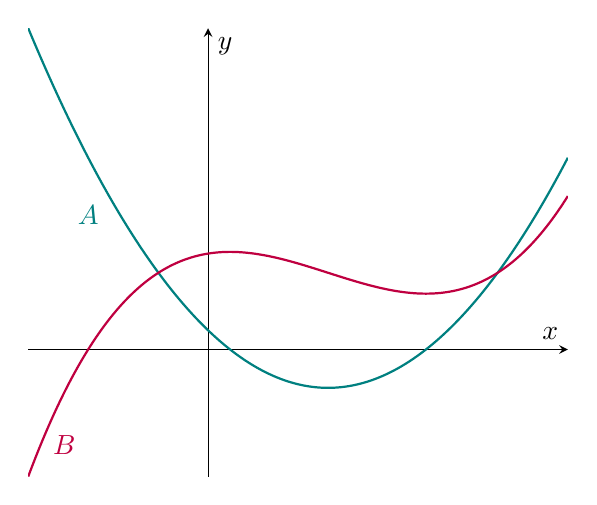
\begin{tikzpicture}
			\begin{axis}[
			axis lines = middle, 
			xlabel = {$x$},
			ylabel = {$y$},
			xmin = -1.5, xmax = 3,
			ticks = none]
				\addplot[color = teal, samples = 1000, thick, domain = -1.5:3] 										{3*x^2-6*x+1 };
				\addplot[color = purple, samples = 1000, thick, domain = -1.5:3] 									{x^3-3*x^2+x+5};
				\node[color = teal] at (axis cs: -1,7) {$A$};
				\node[color = purple] at (axis cs: -1.2,-5) {$B$};
			\end{axis}
		\end{tikzpicture}
		\caption{Grafer for $f$ og $f'$}
		\label{fig:grafer}
\end{figure}
\phantom{h}
\end{opgavetekst}
\begin{delopgave}{(10 point)}{1}
	Afgør hvilken af graferne \textit{\color{teal} A} og \textit{\color{purple} B} der tilhører $f$ og hvilken der tilhører $f'$. 
	Begrund dit svar. 
\end{delopgave}

%%%%%%%%%%%%%%%%%%%%%%%%%%%%%%%%%%%%%%%%%%%%%%%%%%%%%%%%%%%%%%%%%%%%%%%
%							Ny Opgave!!!!!							%
%%%%%%%%%%%%%%%%%%%%%%%%%%%%%%%%%%%%%%%%%%%%%%%%%%%%%%%%%%%%%%%%%%%%%%%

\newpage
\begin{opgavetekst}{Opgave 3}
	En funktion $f$ er givet ved
	\begin{align*}
		f(x) = x^3-6x^2+3.
	\end{align*}
\end{opgavetekst}
\begin{delopgave}{(10 point)}{1}
	Bestem en ligning for tangenten i punktet $P(2,f(2))$. 
\end{delopgave}
%%%%%%%%%%%%%%%%%%%%%%%%%%%%%%%%%%%%%%%%%%%%%%%%%%%%%%%%%%%%%%%%%%%%%%%
%							Ny Opgave!!!!!							%
%%%%%%%%%%%%%%%%%%%%%%%%%%%%%%%%%%%%%%%%%%%%%%%%%%%%%%%%%%%%%%%%%%%%%%%
\begin{opgavetekst}{Opgave 4}
	Differentiér følgende funktioner. 
\end{opgavetekst}
\begin{delopgave}{(7.5 point)}{1}
	$\cos(x)\cdot x^3$.
\end{delopgave}
\begin{delopgave}{(7.5 point)}{2}
	$\ln(x)\cdot \sqrt{x}$.
\end{delopgave}

%%%%%%%%%%%%%%%%%%%%%%%%%%%%%%%%%%%%%%%%%%%%%%%%%%%%%%%%%%%%%%%%%%%%%%%
%							Ny Opgave!!!!!							%
%%%%%%%%%%%%%%%%%%%%%%%%%%%%%%%%%%%%%%%%%%%%%%%%%%%%%%%%%%%%%%%%%%%%%%%
\begin{opgavetekst}{Opgave 5}
	Lad $f$ være givet ved
	\begin{align*}
		f(x) = \frac{1}{3}x^3 +\frac{3}{2}x^2-4x+11
	\end{align*}
\end{opgavetekst}
\begin{delopgave}{(5 point)}{1}
	Bestem $f'(x)$
\end{delopgave}
\begin{delopgave}{(5 point)}{2}
	Løs ligningen $f'(x)=0$. 
\end{delopgave}
\begin{delopgave}{(10 point)}{3}
	Bestem monotoniforholdene for $f$. 
\end{delopgave}
